%%%%%%%%%%%%%%%%%%%%%%%%%%%%%%%%%%%%%%%%%
% 
% LaTeX Template
% Version 3.1 (25/3/14)
%
%%%%%%%%%%%%%%%%%%%%%%%%%%%%%%%%%%%%%%%%%

%----------------------------------------------------------------------------------------
%	PACKAGES AND DOCUMENT CONFIGURATIONS
%----------------------------------------------------------------------------------------

\documentclass[12pt, a4 paper]{article}

\usepackage{tikz}
%\usepackage[top=2cm, bottom=2cm, outer=0cm, inner=0cm]{geometry}
\usepackage{graphicx} % Required for the inclusion of images
\usepackage{multicol} % Required for multicolumns
\usepackage{setspace} % Required for line spacing
\setlength\parindent{0pt} % Removes all indentation from paragraphs
\setlength{\columnseprule}{0.4pt} % Adds vertical line between multicolumns
\usepackage{multirow} % Required for multirows
\usepackage{booktabs} % For prettier tables
\usepackage{xcolor}
%\usepackage{tabularx}
%\renewcommand{\rmdefault}{ptm}

%\usepackage{helvet}

\usepackage{times} % Uncomment to use the Times New Roman font

%----------------------------------------------------------------------------------------
%	DOCUMENT INFORMATION
%----------------------------------------------------------------------------------------

\begin{document}

\tikz[remember picture,overlay] \node[inner sep=0pt] at (current page.center){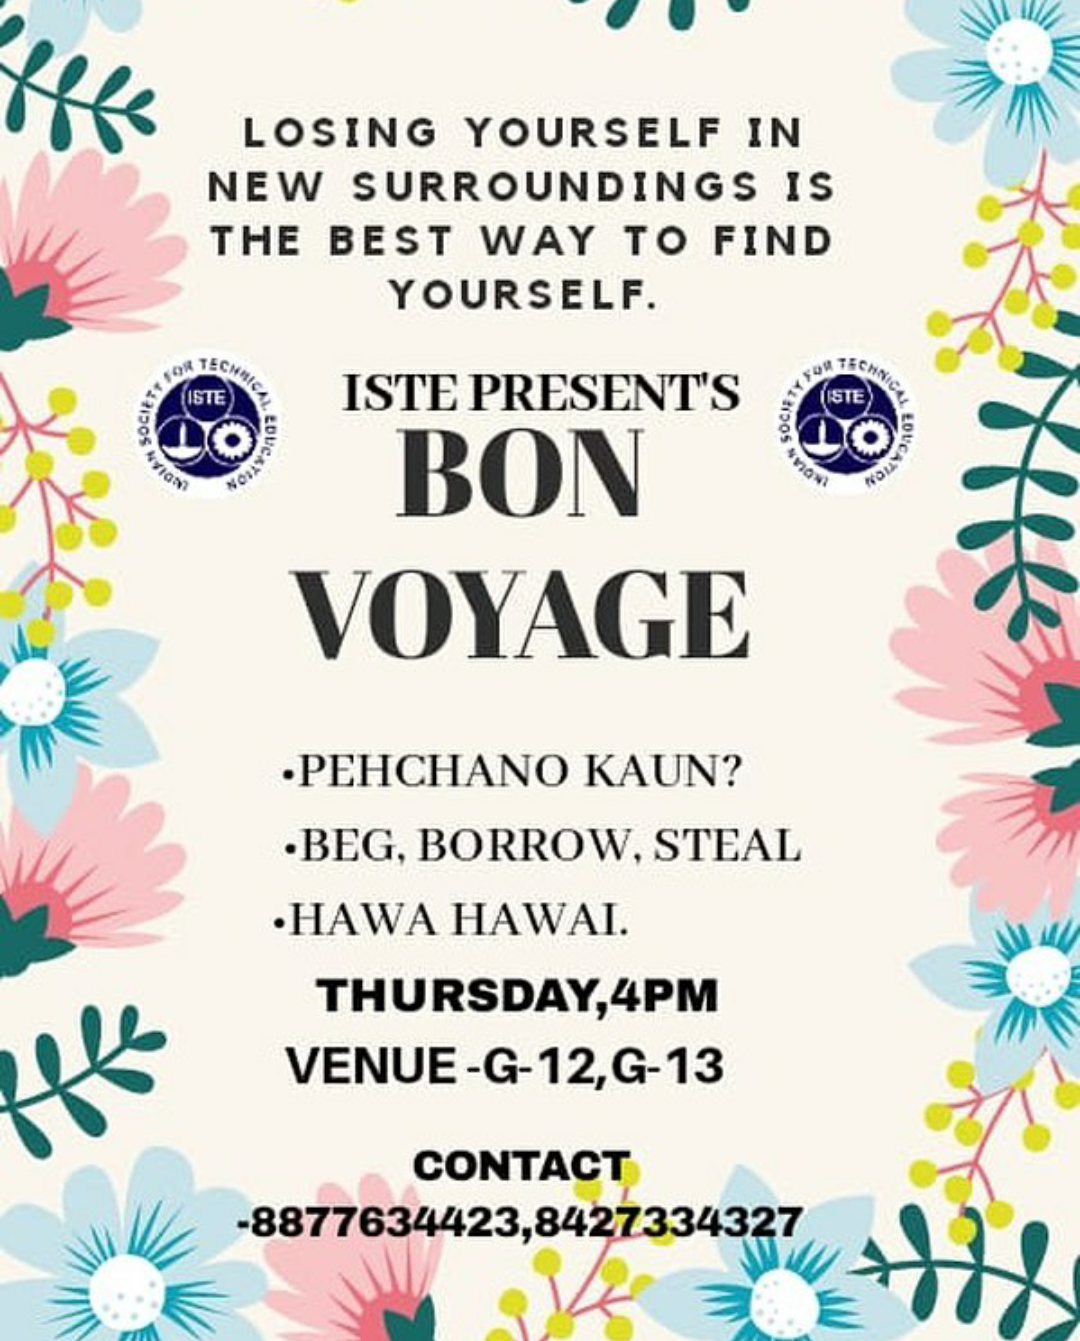
\includegraphics[width=\paperwidth,height=\paperheight]{image.png}};

\clearpage

%\font\myfont=cmr12 at 35pt
%\title{\myfont  Event Name} % Write Event name here
%\author{}
%\date{\vspace{-10ex}}

%\maketitle % Insert the title, author and date
\setstretch{1.5}

%\tikz[remember picture,overlay] \node[opacity=0.8,inner sep=0pt] at (current page.center){
\includegraphics[width=\paperwidth,height=\paperheight]{Border48-A4--Arvin61r58.png}};
%\tikz[remember picture,overlay] \node[opacity=0.5,inner sep=0pt] at (current page.center){\includegraphics[width=\paperwidth,height=\paperheight]{color-2174049__340.png}};

\begin{center}
\Huge \bfseries \ttfamily BON VOYAGE
\end{center}

\begin{center}
\large Event For Interaction With First Year 
\end{center}

\begin{center}
\begin{multicols}{2}
\begin{tabular}{l r}
Date: & 02/08/2018\\ % Date the event was held
Time: & 2:00 pm to 4:00 pm \\ % Time of event 
\end{tabular}
\columnbreak
\begin{tabular}{l r}
Venue: & Auditorium and Nescafe Ground \\ % Venue of event
%Total Attendance: & Number \\ % Number of participants
\end{tabular}
\end{multicols}


\begin{LARGE}
Pehchano kaun?   Beg,Borrow,Steal!!    Hawa Hawai
\end{LARGE}

\begin{Large}
\begin{multicols}{2}
A techno fun event “Bon Voyage” was organized on 2nd August 2018 from 2pm to 4pm at the college auditorium and nescafe ground for interaction with the first year students.

\columnbreak
%\includegraphics[width=\linewidth]{placeholder.jpg}
  %\caption{A boat.}
  %\label{fig:boat1}
\end{multicols}

\begin{multicols}{2}

%\includegraphics[width=\linewidth]{placeholder.jpg}

\columnbreak
The event comprised of three rounds 
ROUND1 (Pehchano Kaun?): In this Event, Students had to recognize the voice played on the projector as well as decipher the picture riddles.

60 students qualified 2nd round.
\end{multicols}

\newpage 

%\tikz[remember picture,overlay] \node[opacity=0.8,inner sep=0pt] at (current page.center){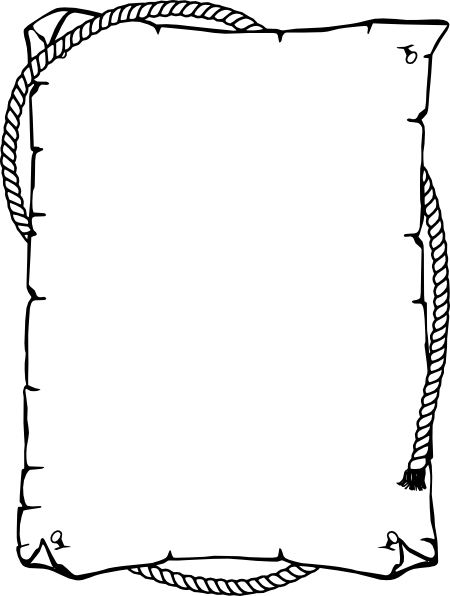
\includegraphics[width=\paperwidth,height=\paperheight]{5TRrp44jc.png}};
%\tikz[remember picture,overlay] \node[opacity=0.8,inner sep=0pt] at (current page.center){\includegraphics[width=\paperwidth,height=\paperheight]{md_5b0912b7c0870.png}};

\begin{multicols}{2}
ROUND2 (Beg,Borrow,Steal): In this round, students had to collect the items mentioned in the list provided to them. Each item was worth some points and the team with maximum points qualified. Top 10 teams got qualified out of 30 Teams and advanced to round 3.

\columnbreak
%\includegraphics[width=\linewidth]{placeholder.jpg}
  
\end{multicols}

\begin{multicols}{2}
%\includegraphics[width=\linewidth]{placeholder.jpg}

\columnbreak
ROUND3(Hawa Hawai): In the third round, participants were divided in teams of 2. Three balloons were given to each team
  
\end{multicols} 

\begin{multicols}{2}
and they had to blow the balloons and move them to the finish line one by one without using their hands. Top three teams wo managed to cross the line won.

\columnbreak
%\includegraphics[width=\linewidth]{placeholder.jpg}
  
\end{multicols} 

\begin{multicols}{2}
%\includegraphics[width=\linewidth]{placeholder.jpg}

\columnbreak
%Some paragraph
  
\end{multicols} 

\end{Large} 
\end{center}

\newpage 

%\tikz[remember picture,overlay] \node[opacity=0.8, inner sep=0pt] at (current page.center){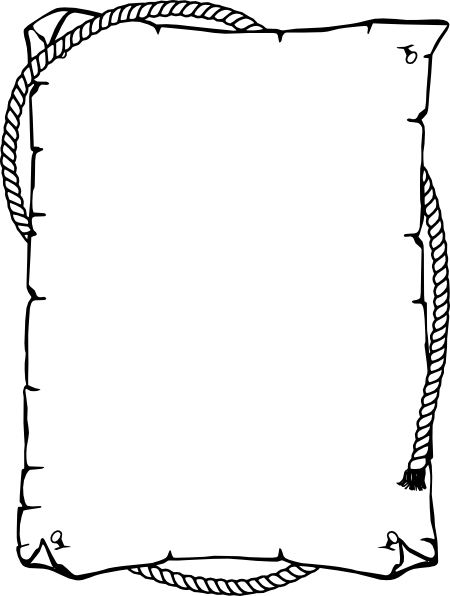
\includegraphics[width=\paperwidth,height=\paperheight]{5TRrp44jc.png}};
%\tikz[remember picture,overlay] \node[opacity=0.8,inner sep=0pt] at (current page.center){\includegraphics[width=\paperwidth,height=paperheight]{md_5b0912b7c0870.png}};

\begin{center}
\Huge Pictures Section
\end{center}

\newpage 

\tikz[remember picture,overlay] \node[opacity=0.8,inner sep=0pt] at (current page.center){
\includegraphics[width=\paperwidth,height=\paperheight]{image1.jpeg}};
\newpage
\tikz[remember picture,overlay] \node[opacity=0.8,inner sep=0pt] at (current page.center){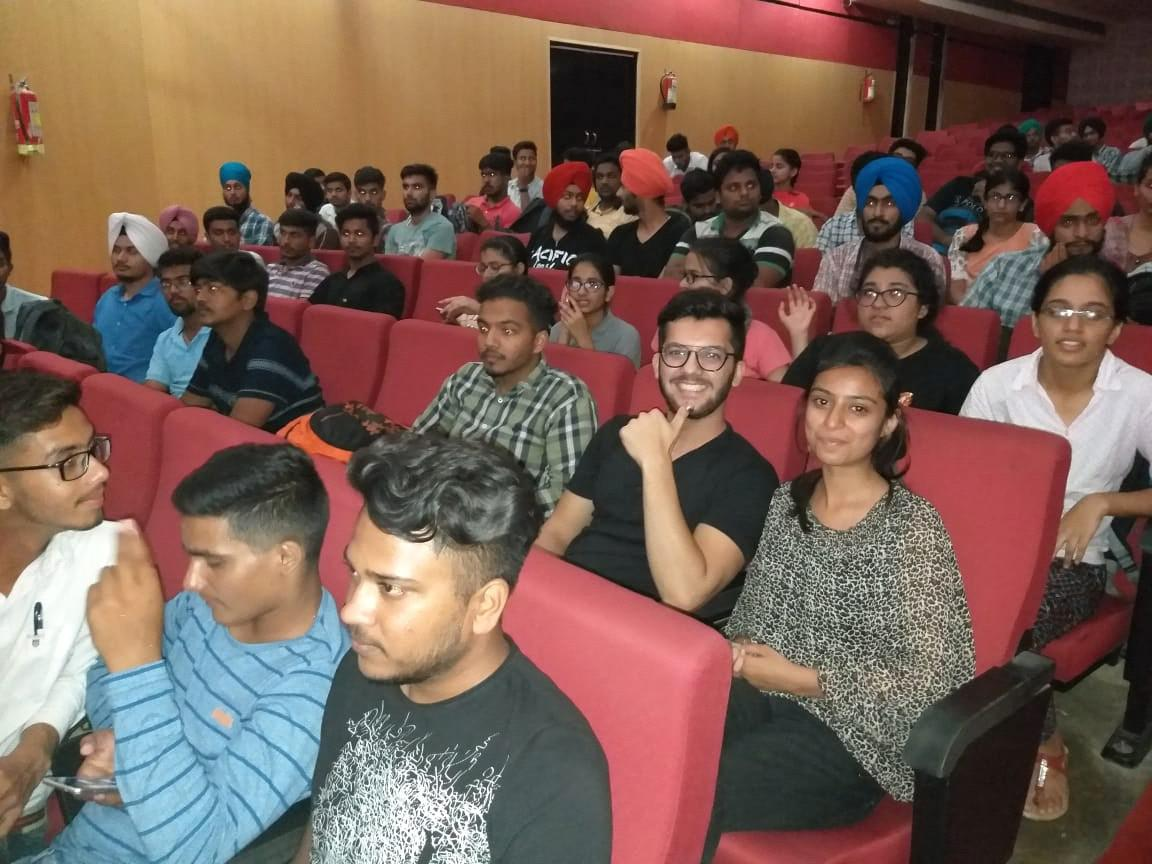
\includegraphics[width=\paperwidth,height=\paperheight]{image2.jpeg}};

\newpage

\begin{center}
\huge Organisers list
\end{center}

\begin{table}[h!]
  \begin{center}
    \begin{tabular}{|c|c|c|c|c|c|} 
    \toprule % <-- Toprule here
      \textbf{S.No.} & \textbf{Name} & \textbf{Branch/Year} & \textbf{Roll No.}\\
      \midrule % <-- Midrule here
      1 & Shubhangi & D2 ECE & 1706782 \\
      2 & Jagmeet Singh & D2 ECE & 1706728  \\
      3 & Dilnish Kaur Bagga & D2 ECE & 1706721  \\
      4 & Harmanjot Kaur & D2 ECE & 1706726 \\
      5 & Tushar Chauhan & D2 ME & 1706533 \\
      6 & Jaskirat Pal Singh & D2 civil & 1706221  \\
      7 & Abhik Sehgal & D3 CSE & 1706544 \\
      8 & Ramanpreet Kaur & D3 CSE  & 1706566 \\
      \bottomrule % <-- Bottomrule here
    \end{tabular}
  \end{center}
\end{table}


\begin{center}
\huge Winner's List
\end{center}

\begin{table}[h!]
  \begin{center}
    \begin{tabular}{|c|c|c|c|c|c|} 
    \toprule % <-- Toprule here
      \textbf{S.No.} & \textbf{Name} & \textbf{Branch/Year} & \textbf{Position} \\
      \midrule % <-- Midrule here
      1 & Amritpal Singh  & D1 CE & \multirow{2}{*}{Ist} \\
      2 & Jappanjot Singh & D1 CE \\
      \hline
      3 & Kavish Thakur   & D1 IT & \multirow{2}{*}{2nd} \\
      4 & Vishal Singla   & D1 CE \\
      \hline
      5 & Gaurav Sharma   & D1 ME & \multirow{2}{*}{3rd} \\
      6 & Aryan Sharma    & D1 ME \\
      \bottomrule % <-- Bottomrule here
    \end{tabular}
  \end{center}
\end{table}

\newpage

\tikz[remember picture,overlay] \node[opacity=0.8,inner sep=0pt] at (current page.center){
\includegraphics[width=\paperwidth,height=\paperheight]{image3.jpeg}};
%\tikz[remember picture,overlay] \node[opacity=0.8,inner sep=0pt] at (current page.center){\includegraphics[width=\paperwidth,height=\paperheight]{md_5b0912b7c0870.png}};


\end{document}